\chapter{Design}
This chapter presents the design choices made to address the requirements outlined in \cref{chap:requirements}. The system is composed of several integrated components, as illustrated in \cref{fig:baseArchDiag}, and described in more detail in \cref{fig:fullArchDiag}:
\begin{itemize}
    \item A set of \textbf{smart contracts} responsible for all blockchain-related operations, including \acrshort{sw} creation and transaction management (see \cref{sec:smartContractsDesign}).
    \item A \textbf{browser extension} that allows students to manage their academic wallets (see \cref{sec:browserExtensionDesign}).
    \item A \textbf{\acrfull{sdk}} designed for universities to interact with the \acrshort{ew} system (see \cref{sec:sdkDesign}).
    \item An external \textbf{decentralized storage system} used to store and retrieve certification files (see \cref{sec:decStorageDesgn}).
\end{itemize}
\begin{figure}
  \centering
  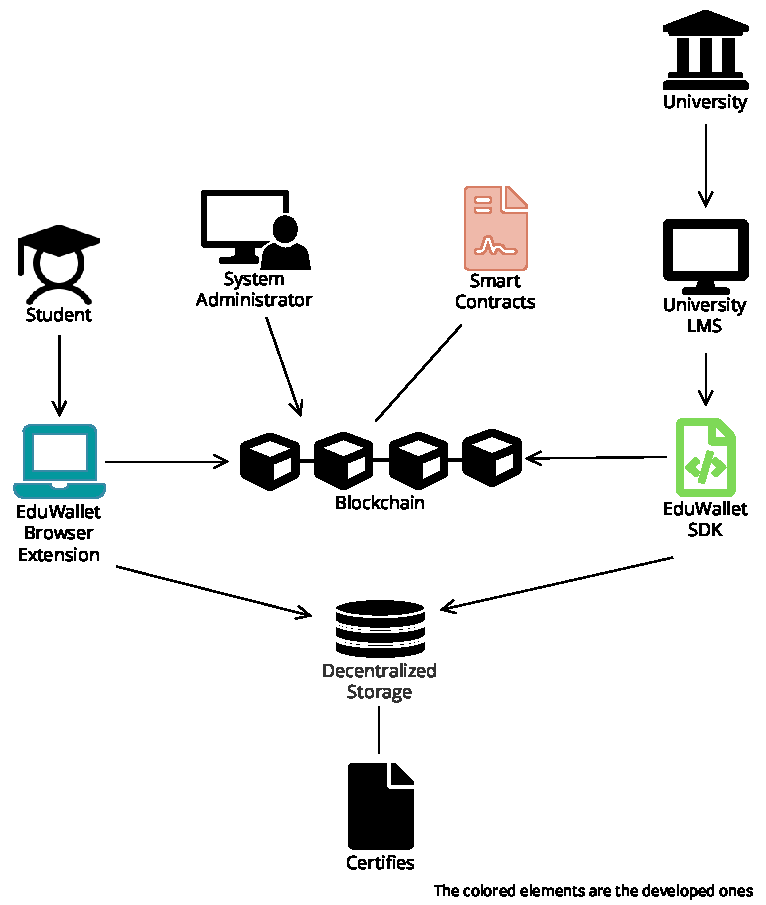
\includegraphics[width=0.6\textwidth]{figures/Architecture diagram basic.pdf}
  \caption[System basic architecture diagram]{Base architecture of the \acrlong{ew} system}
  \label{fig:baseArchDiag}
\end{figure}
In addition to these core components, we developed a simple yet complete \textbf{\acrfull{cli}}, which simulates a university's \acrshort{lms} and its interaction with the academic records system. The \acrshort{cli} serves as a testing and demonstration tool and enables users to perform all operations typically available to universities, thereby simplifying the interaction with our \acrshort{sdk}.

Since the focus of our work is on the interaction of universities and students with the academic registry, the system administrator's core functionalities\footnote{The approval and subscription of universities} have been inserted directly in the \acrshort{cli}. This design decision streamlines our use case and reduces unnecessary complexity.

A more detailed analysis of each component is provided in the following sections.

\begin{figure}[htpb]
  \centering
  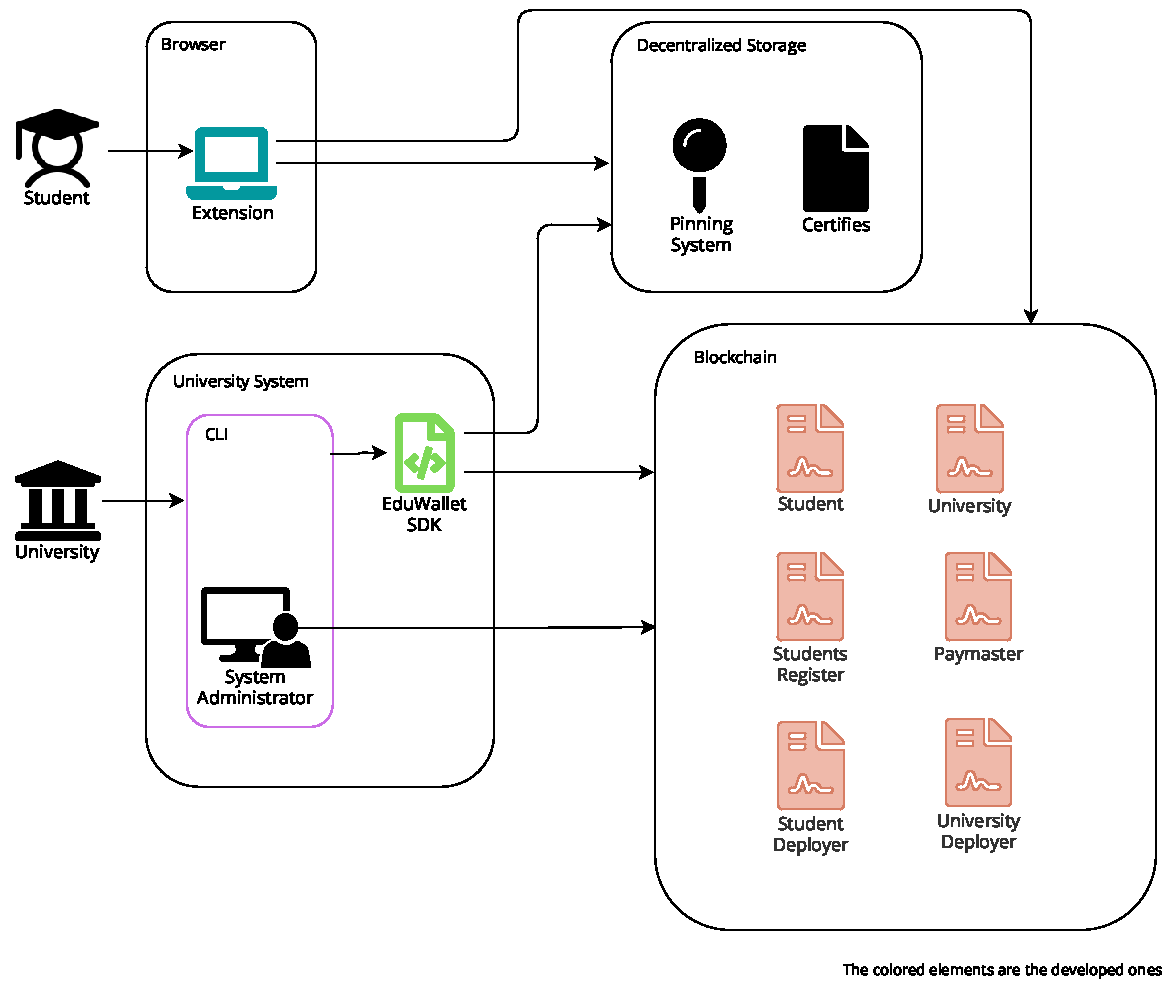
\includegraphics[width=0.8\textwidth]{figures/Architecture diagram complete.pdf}
  \caption[System architecture diagram]{Complete architecture of the \acrlong{ew} system}
  \label{fig:fullArchDiag}
\end{figure}

\section{Smart Contracts}
\label{sec:smartContractsDesign}
This section presents the design choices underlying the development of the smart contracts, which constitute the core logic of the \acrshort{ew} system. These contracts enable secure and decentralized management of the platform by leveraging blockchain principles such as wallets, transactions, and advanced mechanism like access control. They manage the creation of student and university accounts, permissions, access to academic records, and data retrieval. Both the browser extension and the \acrshort{sdk} interact with these contracts to provide users with the necessary functionalities, using TypeScript libraries, such as \textit{ethers}\footnote{\url{https://docs.ethers.org/v6}} for seamless integration.

\subsection{Blockchain Platform and Technologies}
The development of a blockchain-based system begins with the selections of a suitable blockchain platform. We selected \acrlong{eth}, a public blockchain known for its extensive developer community and rich ecosystem of features particularly suitable for an academic record systems \cite{mustafa2024publiceduchain}\cite{yassynzhanbolatzhan2021verificationuniversitystudent}. \acrlong{eth} supports smart contract development in multiple languages and serves as the foundation for various layer 2 solutions that enhance performance and scalability. This flexibility allows the system to be initially developed for the \acrlong{eth} mainnet and later migrated to a layer 2 chain to take advantage of specific features, with minimal development overhead. Notable \acrlong{eth}-based layer 2 solution include:

\begin{itemize}
    \item \textbf{Polygon}, offering faster and more cost-efficient transactions than the Ethereum mainnet.
    \item \textbf{Arbitrum}, improving scalability while maintaining compatibility with Ethereum smart contracts.
    \item \textbf{ZKsync}, ensuring high security and rapid finality through validity proofs.
    \item \textbf{Optimism}, emphasizing simplicity and seamless integration with the Ethereum ecosystem.
    \item \textbf{Starknet}, introducing its own high-performance language, Cairo\footnote{\url{https://www.cairo-lang.org/}}, optimized for zero-knowledge computation.
\end{itemize}

For the implementation, we selected Solidity\footnote{\url{https://soliditylang.org/}} as the programming language. Solidity is an object-oriented language, designed specifically for writing smart contracts on \acrlong{eth} and the \acrshort{evm}, influenced by C++, JavaScript and Python\footnote{\url{https://github.com/ethereum/solidity/blob/develop/docs/index.rst}}. It is the most widely adopted language in the \acrlong{eth} ecosystem, supported by and active and large developer community. Give our prior experience with Solidity, this choice was natural and well-suited to our objectives.

\subsection{Architecture}
\begin{figure}
  \centering
  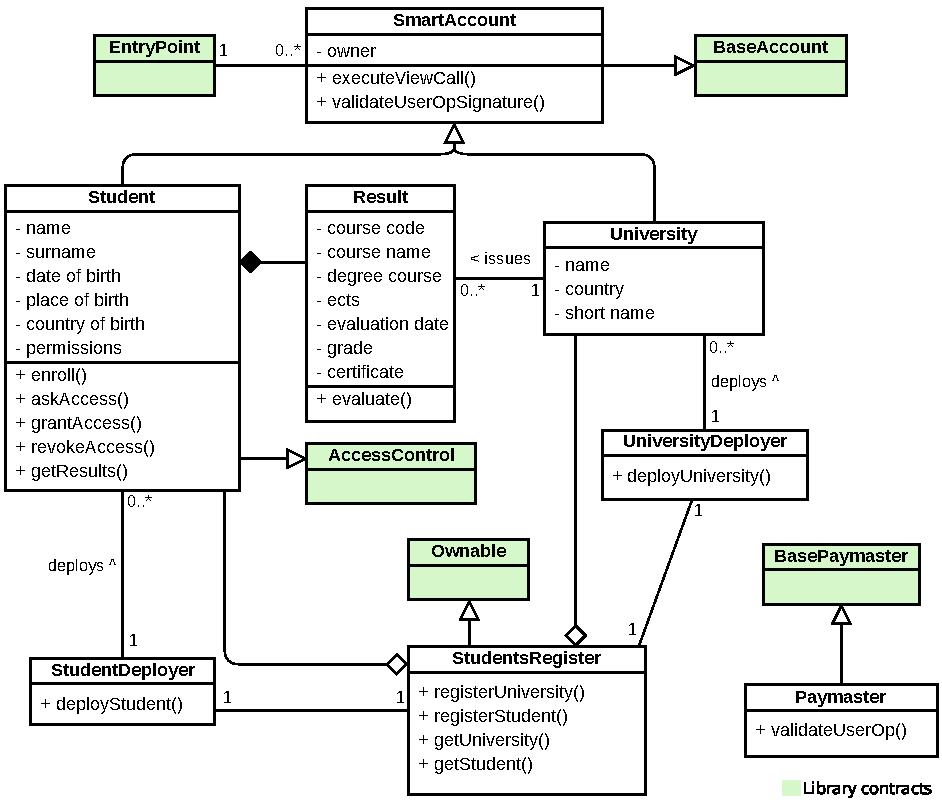
\includegraphics[width=1\textwidth]{figures/Contracts class diagram.pdf}
  \caption[Smart contracts architecture class diagram]{Class diagram representing smart contracts architecture}
  \label{fig:contractsClass}
\end{figure}

The overall architecture of the system is illustrated in the class diagram in \cref{fig:contractsClass}. The \acrshort{ew} system is composed of seven custom smart contracts, represented as white classes in the diagram. (\textit{Result} is not a smart contract, see \cref{sssec:studentContract} for more details). 

\begin{enumerate}
    \item \textbf{SmartAccount}: Defines the structure of a smart account following the account abstraction protocol.
    \item \textbf{Student}: Represents an individual student in the system.
    \item \textbf{University}: Represents a university entity.
    \item \textbf{StudentDeployer}: Responsible for deploying \textit{Student} contracts.
    \item \textbf{UniversityDeployer}: Deploys \textit{University} contracts.
    \item \textbf{StudentsRegister}: Manages and stores information about students and universities.
    \item \textbf{Paymaster}: Sponsors blockchain transactions made by students and universities.
\end{enumerate}
It addition, the system relies on four external contracts, shown in green in \cref{fig:contractsClass}, which are derived form established libraries such as \textit{OpenZeppelin}\footnote{https://openzeppelin.com/}:
\begin{enumerate}
    \item \textbf{EntryPoint}: A singleton contract that receives transactions from smart accounts and executes user operations.
    \item \textbf{AccessControl}\footnote{\url{https://docs.openzeppelin.com/contracts/5.x/access-control}}: Provides a comprehensive role-based access control mechanism.
    \item \textbf{BaseAccount}: Abstract contract defining the core behaviors of a smart account under the account abstraction protocol.
    \item \textbf{BasePaymaster}: Abstract contract defining the structure of a paymaster that sponsors user transactions.
\end{enumerate}

\subsubsection{SmartAccount}

\subsubsection{Student}
\label{sssec:studentContract}
The \textit{Student} contract encapsulates the majority of the system's logic. Its primary responsibilities include storing the student's personal information, such as name, surname, date of birth, place of birth and country of birth, as well as managing their academic records. These records are stored using the structure presented in \cref{lst:resultStruct}. 
\lstinputlisting[
    caption={\textit{Result} structure within the \textit{Student} smart contract},
    label=lst:resultStruct,
    language=Solidity,
]{listings/result.sol}
Due to Solidity's limited support for floating-point numbers, and because the \acrshort{ects} credits may not always be whole number, the \acrshort{ects} value is stored as the original number multiplied by 100. The type \textit{uint16} is used for this purpose, allowing values up to 655.36\footnote{The maximum number representable with 16 bits is 65536},  which is more than sufficient for academic credit systems. A smaller unsigned integer type, such as \textit{uint8}, supports only values from 0 to 2.55 in this context, which is clearly inadequate. The field \textit{certificateHash} stores the CID of the certificate, acting as a reference to its location in the decentralized storage system (see BACKGROUND\_IPFS and \cref{sec:decStorageDesgn} for further explanation). 

Additional functionalities, all addressing \textit{FR 5} in \cref{tab:funcReq}, include enabling universities to:
\begin{itemize}
    \item Retrieve a student's personal and academic information.
    \item Enrol the student in a new course.
    \item Record and evaluation for course the student has already attended.
\end{itemize}
All such interactions are governed by a strict access control mechanism, implemented to fulfill the relevant functional requirements outlined in \cref{tab:funcReq}, namely \textit{FR 6}, \textit{FR 7}, and \textit{FR 12}. This mechanism is based on the \textit{AccessControl} library, specifically the \textit{AccessControlEnumerable} variant, which enables the definition of roles and their association with specific addresses. Within the \textit{Student} contract, four distinct roles are defined:

\begin{enumerate}
    \item \textbf{reader}
    \item \textbf{writer}
    \item \textbf{reader requester}
    \item \textbf{writer requester}
\end{enumerate}
These roles cover all possible scenarios. When an institution requests read or write access to a student's academic records,  its smart account address is assigned the corresponding role. Since \textit{AccessControlEnumerate} supports enumeration of role bearers, the student can query and view which institutions have pending access requests. When an institution attempts to access or modify a student's academic records, the \textit{Student} contract verifies whether the caller's address has been granted the appropriate role, thereby enforcing access restrictions. This mechanism requires the \textit{Student} contract to support a set of permission management functions, including the ability for students to grant, revoke, and inspect permissions (\textit{FR 12}), as well as for universities to request and verify their access rights (\textit{FR 7}).

As shown in \cref{fig:useCaseCli}, \textit{Student} contracts are deployed by the \textit{StudentDeployer}, which is invoked by the \textit{StudentsRegister} contract when a university registers a new student in the \acrshort{ew} system. Upon registration, the initiating university is automatically granted write permissions for the student's academic record, reflecting its role as the enrolling institution responsible for issuing evaluations. All subsequent interactions with the \textit{Student} contract are carried out either by the browser extension or the \acrshort{sdk}. The browser extension is responsible for retrieving personal and academic data and managing permissions on the student's behalf. The \acrshort{sdk}, on the other hand, acts on behalf of universities to access and modify the student's academic wallet. To facilitate these interactions, the \textit{Strudent} contract defines several structured data types, which are used for functions inputs and outputs. These structures improve code readability and usability by grouping related data into cohesive types. Instead of requiring users to  pass multiple separate parameters in a specific order, an approach that increases the risk of errors, developers can simply import the relevant structure and populate its fields. The data type defined in the \textit{Student} contract are:

\begin{itemize}
    \item \textbf{EnrollmentInfo}: Contains the information required to enrol a student in a course; used as input for the enrolment function.
    \item \textbf{EvaluationInfo}: Contains the data needed to record an evaluation; used as input for the evaluation function.
    \item \textbf{Result}: Previously presented, this structure stores the details of a course attended by the student and is used to return the student's academic records.
    \item \textbf{StudentBasicInfo}: Represents the student's personal information.
    \item \textbf{StudentInfo}: A composite structure that includes the \textit{StudentBasicInfo} and a list of \textit{Result} structures, representing the student’s complete academic profile.
\end{itemize}

\subsubsection{University}
Since the primary focus of this work is on the interaction between students and their academic records, as well as the ownership of such data, the institutional accounts (smart accounts) of universities, implemented through the \textit{University} contract, are designed to simpler that those of students. The \textit{University} contract, like \textit{Student}, extends the \textit{BaseAccount} contract, enabling it to function as a smart account compatible with the account abstraction protocol. As a result, universities can use their institutional wallet, via the \acrshort{sdk}, to perform blockchain transactions, which are then sponsored by the \textit{Paymaster}. 

In addition, because universities are identified solely by their contract address in interactions with other smart contracts, the \textit{University} contract also stores descriptive metadata, including the institution's name, country, and a short identifier. Apart from the \textit{UniversityDeployer}, which is responsible for deploying the contract, the only components that interact directly with the \textit{University} contract are the \acrshort{sdk} and the browser extension. When these components need to access university-related information, they do so using the institution's contract address. For instance, when a student retrieves their academic records, each record references the issuing university by it address. The browser extension must then query the blockchain to access the corresponding \textit{University} contract and extract the relevant metadata.    

\subsubsection{StudentDeployer and UniversityDeployer}
The deployment of \textit{Student} and \textit{University} contracts is handled by the \textit{StudentDeployer} and \textit{UniversityDeployer} contracts, respectively. When a system administrator registers a new university, or a university registers a new student through the \acrshort{sdk}, they interact with the \textit{StudentsRegister} smart contract. This contract, in turn, invokes one of the deployer contracts to create the corresponding smart contract instance. This architecture implements the factory pattern, a design principle commonly used in object-oriented programming to abstract the creation of objects. In the context of the \acrshort{ew} system, the deployer contracts abstract and encapsulate the instantiation of new \textit{Student} and \textit{University} contracts.

The adoption of the factory pattern offers several advantages over embedding the deployment logic directly within the \textit{StudentsRegister} contract:

\begin{itemize}
    \item It separates the contract creation logic from the registration logic, improving modularity and maintainability.
    \item It reduces the complexity of the \textit{StudentsRegister} contract by externalizing the deployment process.
    \item It minimizes the contract size of \textit{StudentsRegister}. In Solidity, deploying a contract via the \texttt{new} keyword requires embedding the bytecode of the deployed contract, which increases the size of the calling contract. Since Solidity enforces a maximum contract size of 24576 bytes, including large deployment code directly could exceed this limit. Using external deployer contracts bypass this issue.
\end{itemize}

The decision to centralize deployments through the \textit{StudentsRegister} contract was also motivated by gas efficiency. On blockchain platforms, reducing the number of transactions typically leads to lower gas costs. By combining the deployment of a contract and the registration of its address into a single transaction, the system reduces the overall gas consumption required for onboarding new entities.

\subsubsection{StudentsRegister}

\subsubsection{Paymaster}
One of the system's key feature is that blockchain usage is nearly transparent for users. Students do not directly interact with wallets or perform transactions themselves, and universities only need the private key associated with their \acrshort{eth} account to manage their institutional smart wallet. This level of abstraction is made possible by the \textit{Paymaster}, a smart contract deployed on the blockchain that sponsors all transactions made by users. This design directly readdressing \textit{NFR 5} (see \cref{tab:nonFuncReq}), which emphasizes minimizing the complexity of interactions with the system for end users.

Without the \textit{Paymaster}, the system would require a mechanism to fund user wallets, presenting three primary options:

\begin{enumerate}
    \item Each user funds their own wallet.
    \item Universities fund the wallets of both students and themselves.
    \item The \acrshort{ew} system centrally manages and funds all wallets.
\end{enumerate}
Each approach has significant drawbacks. The first and second require users to manage cryptocurrency wallets and purchase tokens, which increases complexity and cost, especially burdensome for students. The third alternative still introduces administrative overhead and security concerns related to managing a large number of wallets.

Our solution utilizes a \textit{Paymaster} that implements the \textit{BasePaymaster} abstract contract, developed as part of the ERC-4337 protocol\footnote{\url{https://www.erc4337.io/}}. For simplicity, our current implementation sponsors all user operations (transactions) it receives, without validating their origin or gas cost. The only enforced constraint, inherited from \textit{BasePaymaster}, is that transactions must be routed through a known \textit{EntryPoint} contract.
This configuration is suitable for testing environments such as local or test networks, where there is no risk of losing real tokens. In a real-world deployment, a more robust implementation would be necessary, specifically, one that integrates with the \textit{StudentsRegister} contract to verify that the transaction sender is a verified student or university. 

\section{Browser Extension}
\label{sec:browserExtensionDesign}

\section{Software Development Kit}
\label{sec:sdkDesign}

\section{Decentralized Storage System}
\label{sec:decStorageDesgn}
This section presents our solution to one of the most significant challenges in blockchain-based systems: the high cost of on-chain storage. To address this issue, we introduce an off-chain decentralized storage solution in our project. This system is used to store and retrieve certification files, such as language certificates or graduation diplomas, which require significantly more space than plain text\footnote{PDF files typically range from a few kilobytes to several megabytes, whereas plain text data usually occupies only a few bytes.}. Storing such documents directly on-chain would result in substantial gas costs, making the approach impractical. 

\subsection{Why a decentralized storage?}
We chose a decentralized storage system over traditional local or cloud-based solutions to maintain the decentralized nature of our environment and to meet the non-functional requirements outlined in \cref{sec:nonFunctionalRequirements}. Among the various decentralized options available, we selected \acrfull{ipfs} for its ability to provide verifiable and distributed file storage. This choice is motivated by several factors: \acrshort{ipfs} is an open source protocol with a large and active community, strong support, and widespread adoption. It also serves as the foundational layer for many other decentralized platforms, such as Filecoin\footnote{\url{https://filecoin.io}} and Web3.Storage\footnote{\url{https://web3.storage}}, allowing future extensions or upgrades to be implemented with minimal effort \cite{erikflorian2022ipfsandfrineds}. Furthermore, \acrshort{ipfs} ensures immutability of stored files, a critical feature for academic certificates, which must remain unchanged over time.

\subsection{Pinning files}
To fully leverage \acrshort{ipfs}, we integrated Filebase\footnote{\url{https://filebase.com}}, a third-party pinning service. Pinning refers to the act of instructing a node to keep a copy of a file permanently, preventing it from being removed during garbage collection. Without Filebase, we would have needed to run our own local \acrshort{ipfs} node and manage file pinning manually, an approach that introduces instead complexity, higher maintenance costs, and reduced data availability in a testing system like ours. In contrast, Filebase handles node operation and file pinning, offering an accessible solution thorough its AWS S3-compatible \acrshort{api}, which simplifies file uploads to the peer-to-peer network. Notably, Filebase also provides a free tier allowing up to 5 GB of storage, which is sufficient for our needs. This is an advantage over other pinning solutions such as Web3.Storage, which lacks a fully free plan, or Pinata\footnote{\url{https://pinata.cloud}}, which offers more limited options.

\subsection{Integration in the system}
As shown in \cref{fig:fullArchDiag}, both the browser extension and the \acrshort{sdk} interact with the storage system. The browser extension retrieves certificate associated with academic records using the official \acrshort{ipfs} public gateway. It presents students with a direct link to each certificate, composed by the gateway's base \acrshort{url} followed by the file's \acrfull{cid} on the \acrshort{ipfs} network. The \acrshort{cid} of each document is stored on-chain within the student's academic wallet, alongside other record information such as the course name (see \cref{sssec:studentContract}). This enables students to view and download their certificates from a standard web interface.

% TODO: Add photo of the extension where you can see the link of a certification
Similarly, the \acrshort{sdk} uses the same mechanism to retrieve certificates on behalf of universities. When uploading a file, however, the \acrshort{sdk} interacts directly with Filebase to ensure the file is pinned and hosted by an active node. The \acrshort{sdk} receives the document from the university, then uses the AWS S3-compatible \acrshort{api} to upload it. The \acrshort{api} requires the key associated with the pinning account (managed by the \acrshort{ew} system administrator) and the file itself. In return, it provides the \acrshort{cid}, which is then stored in the academic record.
% TODO: Reference implementation section

\subsection{Security and Limitations}
Academic certifies, and official documents more broadly, are legal artifacts that must always be secure and verifiable. \acrshort{ipfs} inherently supports these properties through its use of content-based addressing. In this model, each file is identified by a \acrshort{cid}, which is derived from the cryptographic hash of the file's content. Any alteration to the file results in a completely different \acrshort{cid}, ensuring that tampering is immediately detectable \cite{benet2014ipfscontentaddressed}. Since the the \acrshort{cid} is stored on the blockchain at the time the certificate is issued by the university, the document's authenticity and integrity are guaranteed.

While \acrshort{ipfs} offers strong immutability and verifiability, it lacks built-in access control. In the context of our system, we assume that certificates are publicly accessible documents. Consequently, any part in possession of a file's \acrshort{cid} can retrieve it via the public gateway. However, if access control becomes a requirement, there are several strategies to address this limitation \cite{barbaraanrealaura2021datapersistence}. One option is to encrypt files before uploading them to \acrshort{ipfs}, such that only authorized components within our system can decrypt them. Another approach is to use a private \acrshort{ipfs} network, where access can be restricted to approved entities. The trade-offs and potential implications of such private deployment will be discussed in the FUTURE WORK CHAPTER.

\section{CLI}
\label{sec:cliDesign}
\begin{figure}
  \centering
  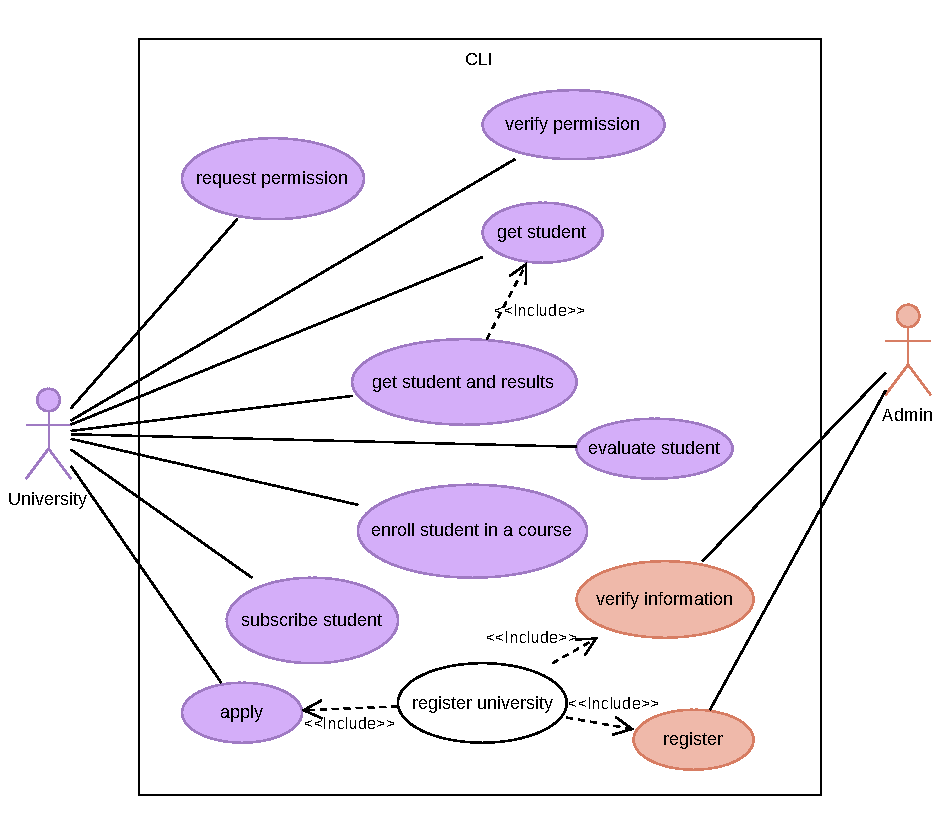
\includegraphics[width=0.8\textwidth]{figures/CLI use case diagram.pdf}
  \caption[\acrshort{cli} use case diagram]{Use case diagram representing the functionalities provided by the \acrshort{cli}.}
  \label{fig:useCaseCli}
\end{figure}
This section describes the testing tool developed to evaluate the use of the \acrshort{sdk}. In a real-world deployment, universities are expected to integrate the \acrshort{sdk} into their existing \acrshort{lms} to interact with \acrlong{ew}. However, given that this is a testing environment, smaller and simpler than a real-world deployment, we developed a minimal \acrlong{cli} to simulate the interaction between a university's system and our academic register. We opted to implement a CLI rather than a web application or desktop GUI and this decision allowed for faster development, enabling us to focus on the core functionalities of the \acrshort{sdk}, the blockchain logic, and the browser extension, without introducing additional complexity related to graphical or \acrfull{ux} design.

\cref{fig:clifigs} illustrates the visual aspects of the \acrshort{cli}. In \cref{sfig:cliDesign1}, users can navigate through a sliding menu offering various options. When input is required, the interface prompts the user for the necessary information and provides visual feedback upon completion of the operation (\cref{sfig:cliDesign2}).The \acrshort{cli} leverages the \textit{inquirer}\footnote{\url{https://www.npmjs.com/package/inquirer}} TypeScript library to manage user interactions and uses \textit{ora}\footnote{\url{https://www.npmjs.com/package/ora}} to display feedback. Specifically, \textit{ora} is responsible for showing success and error messages, as well as animated text with spinners to indicate ongoing operations.

\begin{figure}
    \centering
    \begin{subfigure}{.5\textwidth}
        \centering
        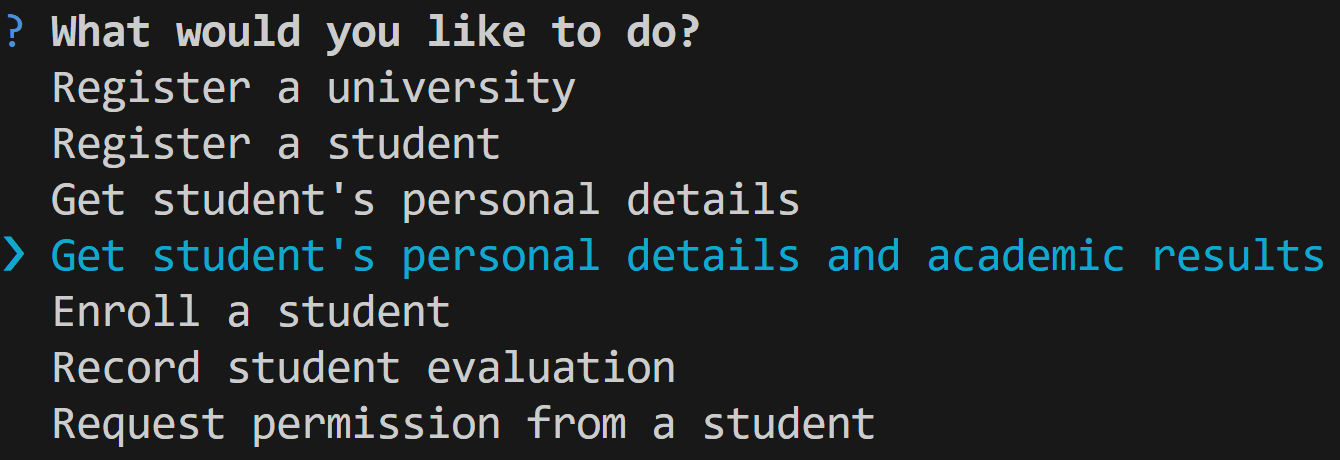
\includegraphics[width=\textwidth]{figures/CLI screen 1.png}
        \caption{Sliding menu}
        \label{sfig:cliDesign1}
    \end{subfigure}
    \hfill
    \begin{subfigure}{.60\textwidth}
        \centering
        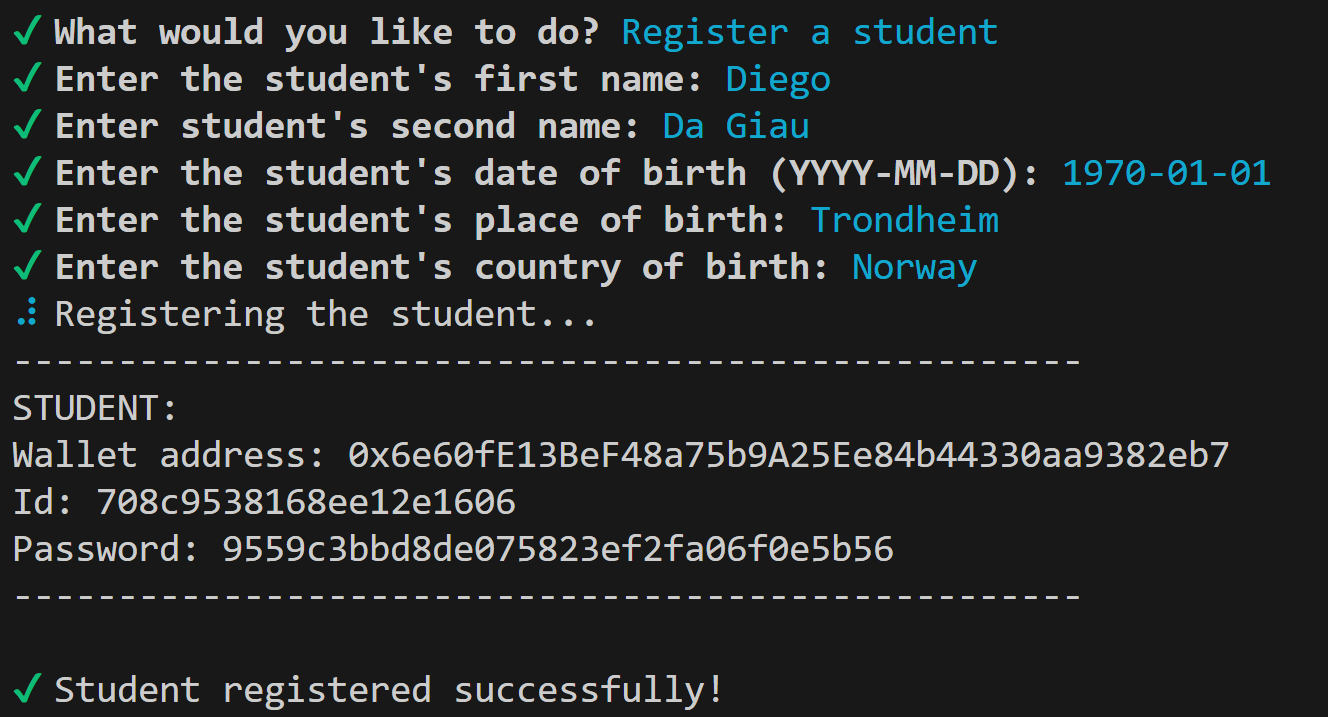
\includegraphics[width=\textwidth]{figures/CLI screen 2.png}
        \caption{User input and visual feedbacks}
        \label{sfig:cliDesign2}
    \end{subfigure}
    \caption[Different aspects of the \acrshort{cli} interface.]{Snapshots of the \acrshort{cli} interface}
    \label{fig:clifigs}
\end{figure}

\subsection{Functionalities}
The \acrshort{cli} exposes all the functionalities outlined in \cref{fig:useCaseCli}. Users can:
\begin{itemize}
    \item Submit a request to register a university in the \acrshort{ew} system.
    \item Register a new student.
    \item Retrieve a student’s personal details.
    \item Retrieve a student’s details and academic results.
    \item Enrol a student in a new course.
    \item Evaluate a student.
    \item Request permissions from a student.
    \item Verify existing permissions.
\end{itemize}
Additionally, the \acrshort{cli} provides options to change the current university and exit the program.

\subsubsection{Testing environment initialization}
Before performing any operation, the \acrshort{cli} must initialize a local blockchain test network by deploying the following smart contracts:
\begin{itemize}
    \item \textit{EntryPoint}
    \item \textit{StudentDeployer}
    \item \textit{UniversityDeployer}
    \item \textit{Paymaster}
    \item \textit{StudentsRegister}
\end{itemize}
The \textit{Paymaster} contract then must also be funded to sponsor transactions on behalf of users.

In public testnets or in production networks, this step would be unnecessary, as the contracts would already be deployed. Their addresses would be hardcoded in the \acrshort{cli}, \acrshort{sdk} and browser extension.

\subsubsection{University registration}
\label{sssec:applyEw}
To apply to the \acrshort{ew} system, a university must provide its name, country, and short name. Upon completion, it receives the private key of the wallet that owns its smart account. This key is used by the \acrshort{cli} to generate the university's \acrlong{eth} wallet, which is then stored as the current active university. In a real \acrshort{lms}, the private key must be securely stored and used to initialize the wallet and use the \acrshort{sdk}. 

To interact with the \textit{EntryPoint}  contract in the local testnet, the \acrshort{cli} also funds the university's \acrshort{eth} wallet. In public or production networks, this is not necessary, as the bundler pays the transaction fees and is reimbursed by the \textit{Paymaster}.

\subsubsection{Register a new student}
To register a student, the  university provides their name, surname, date of birth, place of birth and country of birth. The \acrshort{cli} then calls the \acrshort{sdk} to create the student's academic wallet and credentials, which are returned to the university (\cref{sfig:cliDesign2}). The academic wallet address uniquely identifies the student and must be stored by the university, as it is required for all future interactions. 

As discussed in the CONTRACT SECTION, universities are responsible for registering students to decentralize the validation process. Since universities already verify student applications, they can provide verified data to the system, avoiding centralization and overloading the system administrator.

The \acrshort{cli} also funds the student's \acrlong{eth} wallet  for local testing. The wallet address is obtained from the login credentials, as done in the browser extension (see BROWSER EXTENSION SECTION).

\subsubsection{Student Information Retrieval}
To retrieve a student's personal information or full academic record, university must provide the student's academic wallet address. The \acrshort{cli} then returns the requested data.

\subsubsection{Enrol and evaluate}
To enrol or evaluate a student, the university must provide the academic wallet address and course code. Enrolment also requires the course name, number of \acrshort{ects} and degree course name (e.g., \textit{Master's in Computer Engineering}, or \textit{Bachelor's in Biology}). Evaluation requires the evaluation date and, optionally, the path to a certificate file. Since the \acrshort{sdk} allows enrolment in or evaluation of multiple courses at once, the \acrshort{cli} also supports submitting multiple records in a single command.     

\subsubsection{Permissions: Request and Verification}
To access or modify student's academic records, the university must request permission. The \acrshort{cli} requires the student's wallet address and the type of permission (read or write). As in most systems, write permission implies read access.
The \acrshort{cli} also includes an option to verify whether the university currently has read or write permission for a specific student.

\subsubsection{Changing University and Exiting the \acrshort{cli}}
These functionalities are unique to the \acrshort{cli} and are included for convenience. To change the active university, the user provides the private key of another registered university. To exit the \acrshort{cli}, the user selects the corresponding menu option.

\subsubsection{Administrator Functionalities}
The \acrshort{cli} also includes admin functionalities, to facilitate system testing. Specifically, the administrator can:
\begin{itemize}
    \item Review the information submitted in university registration request.
    \item Approve and register universities in the system.
\end{itemize}
These functionalities are embedded within the university registration option. A university is automatically registered when its information is provided by the user during the registration process.

\subsection{Data validation}
All user input is validated using regular expressions and formatting rules. For instance, wallet addresses and private keys are validated based on length and structure\footnote{Private keys must start with \textit{0x} and be followed by 64 hexadecimal characters; addresses by 42.}. Strings are validated to fall within predefined length limits. Dates must follow the \textit{YYYY-MM-DD} format to avoid ambiguity and must be after January 1, 1970, as they are stored as Unix timestamps (unsigned integers). \acrshort{ects} values are checked to ensure they are valid integers or floating-point numbers within acceptable limits. Since the smart contracts store \acrshort{ects} as integers scaled by 100 (to avoid the issue of Solidity with floating point numbers), the \acrshort{cli} ensures the values will not cause overflow during storage.